\documentclass{article}

\title{Zumobot case study}
\date{29.6.2017}
\author{Javier Reyes \and Hari Kumar Venkatesh}

\usepackage{graphicx}
\usepackage{booktabs}
\usepackage{amsmath}
\usepackage{comment}

\usepackage[backend=biber, style=ieee]{biblatex}
\bibliography{report}


\begin{document}

\maketitle
\pagenumbering{gobble}
\newpage
\pagenumbering{arabic}

\tableofcontents
\newpage

\section*{Introduction}

One of the most used study cases in Control Theory is the Inverted Pendulum analysis, as it presents an unstable open-loop characteristic but is also possible to stabilize it on a closed-loop configuration.

Here we present the analysis of the Zumobot 32U4, a small robot available in the market. The Zumo 32U4 robot is a complete, versatile robot controlled by an Arduino-compatible ATmega32U4 microcontroller. The Zumo 32U4 robot can be programmed from a computer using any operating system that supports the Arduino environment.

TODO: Complete

\section{System analysis}

An inverted pendulum can be represented as a rigid body pendulum connected to a cart moving on a horizontal axis. Controlling the stability of the Zumobot can be compared to balancing the inverted pendulum on the moving cart.

\begin{comment}
	\begin{figure}[!htbp]
		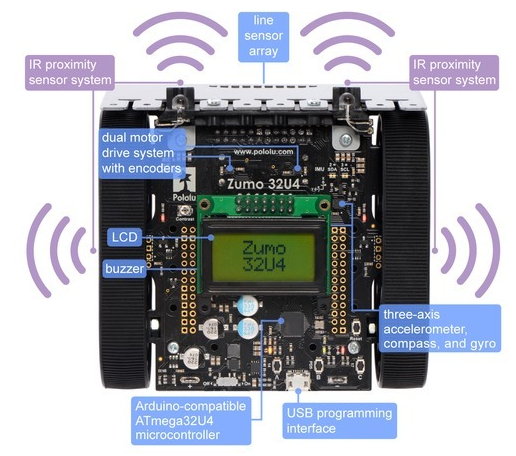
\includegraphics{img/zumo-superior.png}
		\centering
		\caption{Superior view of the zumo robot.}
		\label{fig:sup-zumo}
	\end{figure}
\end{comment}

%The figure \ref{fig:sup-zumo} shows the robot that will be modeled as a Wheeled Inverted Pendulum.

\begin{comment}
	\begin{table}[!htbp]
		\centering
		\caption{Basic table.}
		\label{tab:tab1}
		\begin{tabular}{ccc}

			\toprule

			header A & header B & header C\\

			\midrule

			a & b & c\\
			c & d & e\\
			f & g & h\\

			\bottomrule

		\end{tabular}
	\end{table}
\end{comment}

%Text of the section\footnote{\label{fn1}This is a footnote}.

%Text of the section after the footnote \ref{fn1}.

TODO: Complete

\section{Mathematical development}

Through the numerous literature is possible to find several approaches to obtain a model for the Inverted Pendulum.

To fully model the dynamic behavior of the zumo robot, we need to consider the equations that govern the movement as rigid body.

TODO: Complete

\subsection{First approach - Sum of forces}

The first approach considered here is described in \cite{SUL03}.

\subsubsection{Dynamic behavior}

The equations of motion are obtained from the sum of forces in the cart for the horizontal direction.

\begin{equation} \label{sfch}
F-b\cdot \dot{x}-N=M\cdot \ddot{x}
\end{equation}

Now considering the pendulum itself, the force applied in the horizontal direction due to the momentum of the pendulum is determined as:

\begin{equation} \label{dhfp}
\tau=r\cdot F=I\cdot \ddot{\theta}
\end{equation}

Given the fact that the moment of inertia of a pendulum of mass $m$ is defined as $I=m\cdot L^2$, the previous equation can be rewritten as:

\begin{equation} \label{dhfp2}
F=\frac{I\cdot \ddot{\theta}}{r}=\frac{m\cdot l^2\cdot \ddot{\theta}}{l}=m\cdot l\cdot \ddot{\theta}
\end{equation}

Obtaining the component of the force defined in \ref{dhfp2} in the horizontal direction:

\begin{equation} \label{sfph}
F=m\cdot l\cdot \ddot{\theta}\cdot \cos{\theta}
\end{equation}

Now, the component of the centripetal force acting on the pendulum is similar to the one in \ref{dhfp2}, but the horizontal component of this force is:

\begin{equation} \label{cfph}
F=m\cdot l\cdot \dot{\theta}^2\cdot \sin{\theta}
\end{equation}

Summing the defined forces present in the horizontal direction of the pendulum in \ref{sfph} and \ref{cfph}, we obtain the following expression:

\begin{equation} \label{nfp}
N=m\cdot \ddot{x}+m\cdot l\cdot \ddot{\theta}\cdot \cos{\theta}-m\cdot l\cdot \dot{\theta}^2\cdot \sin{\theta}
\end{equation}

Now we can substitute \ref{nfp} into \ref{sfch}, we obtain the first equation of motion:

\begin{equation} \label{fem}
F=(M+m)\ddot{x}+b\cdot \dot{x}+m\cdot l\cdot \ddot{\theta}\cdot \cos{\theta}-m\cdot l\cdot \dot{\theta}^2\cdot \sin{\theta}
\end{equation}

To get the second equation of motion, we sum the forces perpendicular to the pendulum. The vertical components of this forces are considered here to get:

\begin{equation} \label{sfppv}
P\cdot \sin{\theta}+N\cdot \cos{\theta}-m\cdot g\cdot \sin{\theta}=m\cdot l\cdot \ddot{\theta}+m\cdot \ddot{x}\cdot \cos{\theta}
\end{equation}

To get rid of the $P$ and $N$ terms, sum the moments around the center of gravity of the pendulum:

\begin{equation} \label{smcg}
-P\cdot l\cdot \sin{\theta}-N\cdot l\cdot \cos{\theta}=I\cdot \ddot{\theta}
\end{equation}

Summing up the equations \ref{sfppv} and \ref{smcg}, we obtain the second equation of movement:

\begin{equation} \label{sem}
(I+m\cdot l^2)\ddot{\theta}+m\cdot g\cdot l\cdot \sin{\theta}=-m\cdot l\cdot \ddot{x}\cdot \cos{\theta}
\end{equation}

The obtained equations are non-linear, so they are linearized around the operating point, defined as the top vertical position or $\pi rad$ from the stable equilibrium position. We need also to define a small angle deviation from the top vertical position, so that $\theta=\pi+\phi$.

Under this circunstances, we can deduce that $\cos{\theta}\approx -1$, $\sin{\theta}\approx -\phi$, and $\dot{\theta}^2\approx 0$. Applying this relations into our movement equations, we obtain:

\begin{equation} \label{feml}
F=(M+m)\ddot{x}+b\cdot \dot{x}-m\cdot l\cdot \ddot{\phi}
\end{equation}

\begin{equation} \label{seml}
(I+m\cdot l^2)\ddot{\phi}-m\cdot g\cdot l\cdot \phi=m\cdot l\cdot \ddot{x}
\end{equation}

To obtain the transfer function of the linearized system of equations analytically, we perform the Laplace transform of the system equations:

\begin{equation} \label{fems}
F(s)=(M+m)s^2\cdot X(s)+b\cdot s\cdot X(s)-m\cdot l\cdot s^2\cdot \Phi(s)
\end{equation}

\begin{equation} \label{sems}
(I+m\cdot l^2)s^2\cdot \Phi(s)-m\cdot g\cdot l\cdot \Phi(s)=m\cdot l\cdot s^2\cdot X(s)
\end{equation}

To unify the equations, we solve \ref{fems} for $X(s)$ and then replace it into \ref{sems}, obtaining:

\begin{equation} \label{ecms}
\frac{\Phi(s)}{F(s)}=\frac{m\cdot l\cdot s}{q\cdot s^3+b(l+m\cdot l^2)s^2-m\cdot g\cdot l(M+m)s-b\cdot m\cdot g\cdot l}
\end{equation}

Where:

\begin{equation} \label{dq}
q=(M+m)(l+m\cdot l^2)-(m\cdot l)^2
\end{equation}

Assuming a coefficient of friction as zero, we can represent the equation as:

\begin{equation} \label{efms}
\frac{\Phi(s)}{F(s)}=\frac{K_p}{\frac{s^2}{A_p^2}-1}
\end{equation}

With:

\begin{equation} \label{dka}
K_p=\frac{1}{(M+m)g} ; A_p=\pm \sqrt{\frac{(M+m)m\cdot g\cdot l}{(M+m)(l+m\cdot l^2)-(m\cdot l)^2}}
\end{equation}

\subsubsection{Actuator system}

TODO: Complete

\subsection{Second approach - Euler-Lagrange}

TODO: Complete

\section{System model}

Text of the section.

\section{Regulator}

Text of the section.

\section{Implementation}

Text of the section.

\begin{appendix}
	\newpage
	\listoffigures
	\newpage
	\listoftables
\end{appendix}

\newpage
\printbibliography
\nocite{*}

\end{document}
